
%%%
%%% CHAPTER
%%%
\chapter{Thermodynamics: Introduction and Principles}\label{Chapter:Introduction}
   \begin{shaded}
      \noindent
      At the end of this chapter you should be able to:
        \begin{enumerate}
           \item kk
        \end{enumerate}
   \end{shaded}

%%%
%%% SECTION
%%%
\section{Introduction}\label{Chapter:Introduction:Section:Introduction}
Thermodynamics studies global properties of the matter and the process (\eg thermal, chemical, mechanical, nuclear etc) in which these properties may be altered. The study of thermodynamics may be divided into two main areas, {\it classical} and {\it statistical} thermodynamics. In the latter, matter is assumed to be formed by assemblies of particles (\ie atoms), and properties' changes of each assemble are obtained from quantum mechanics. {\it Classical thermodynamics} studies the macroscopic change of properties, \ie it is assumed that matter is formed by a large quantity of particles' assemblies that has properties representing the interactions between these assemblies. 

In practice, any thermodynamic analysis starts by defining the domain of interest, which can be a volume in space or quantity of matter (Fig.~\ref{Chapter:Introduction:Fig:Domain} a). This domain is called {\it system} and the remaining of the space is called {\it surroundings} (or {\it neighbourhood}) limited by {\it boundaries} . In Fig.~\ref{Chapter:Introduction:Fig:Domain}(b), nitrogen gas is contained in a pressure vessel with prescribed wall thickness. In this case, the interior of the vessel with N$_{2}$ is the {\it system}, whereas the wall (in contact with the gas) is the border of the system.  These 3 components




%%% Figure
      \begin{figure}%
          \vbox{\hbox{
             \hspace{0.cm}\hbox{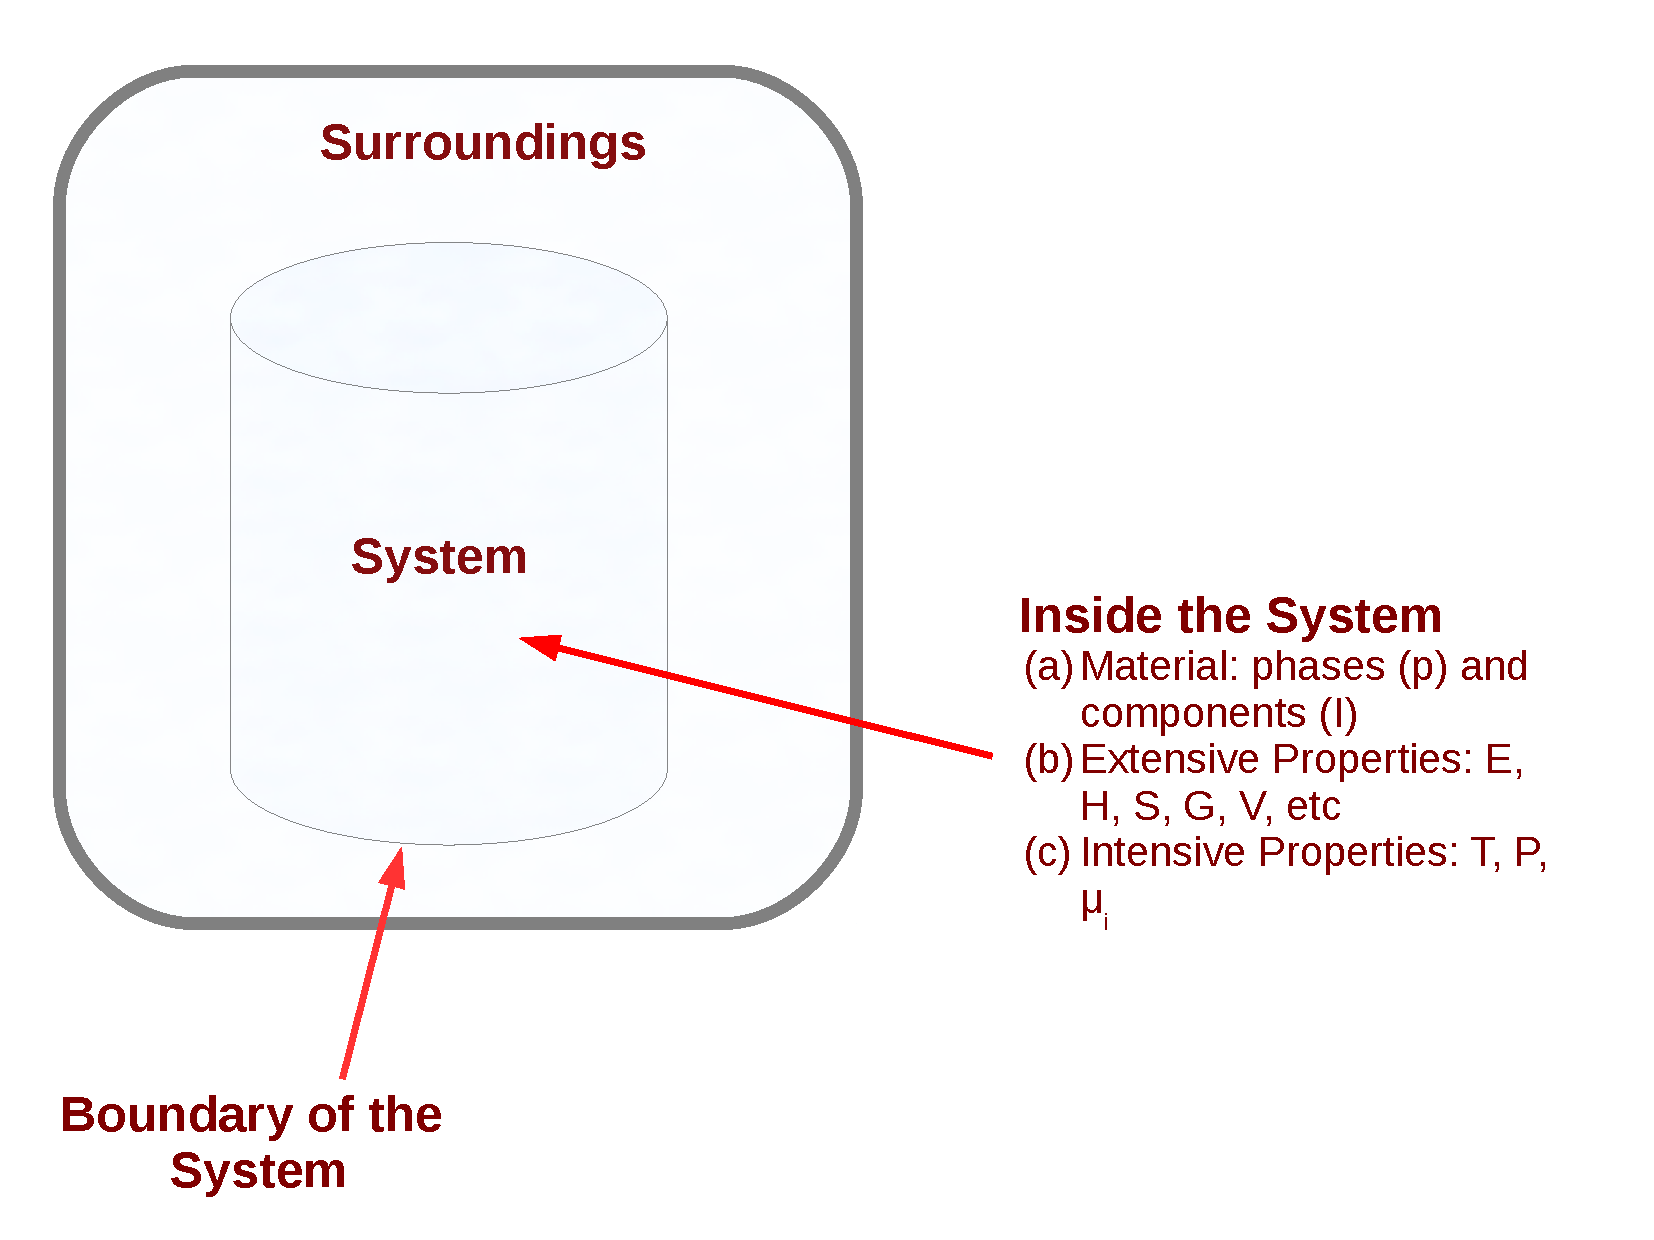
\includegraphics[width=8cm, height=8cm]{./../Pics/Fig_SystemDefinition}}
             \hspace{0.cm}\hbox{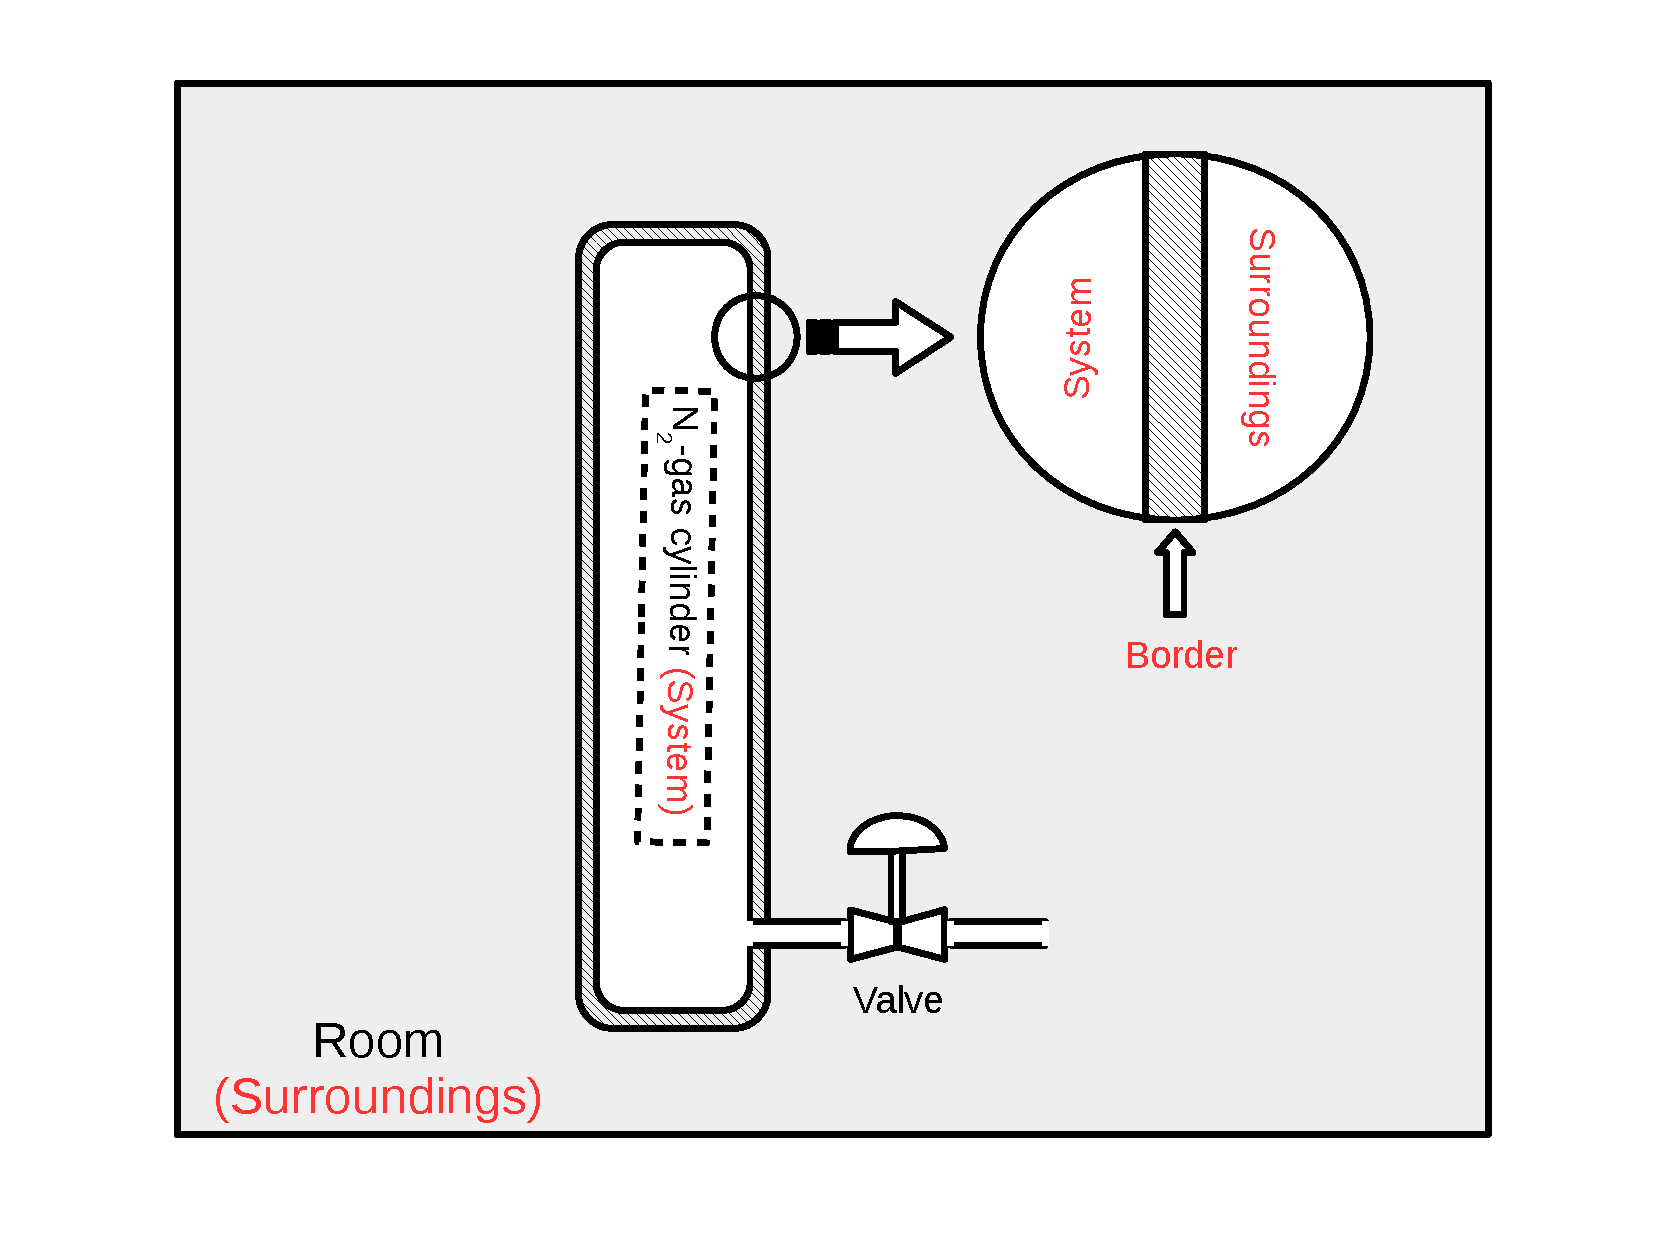
\includegraphics[width=9cm, height=5cm]{./../Pics/Fig_SystemDefinition2}}}
             \vspace{.1cm}
              \hbox{\hspace{3.5cm}(a)\hspace{8cm}(b)}
             \vspace{.5cm}
             \hspace{3cm}\hbox{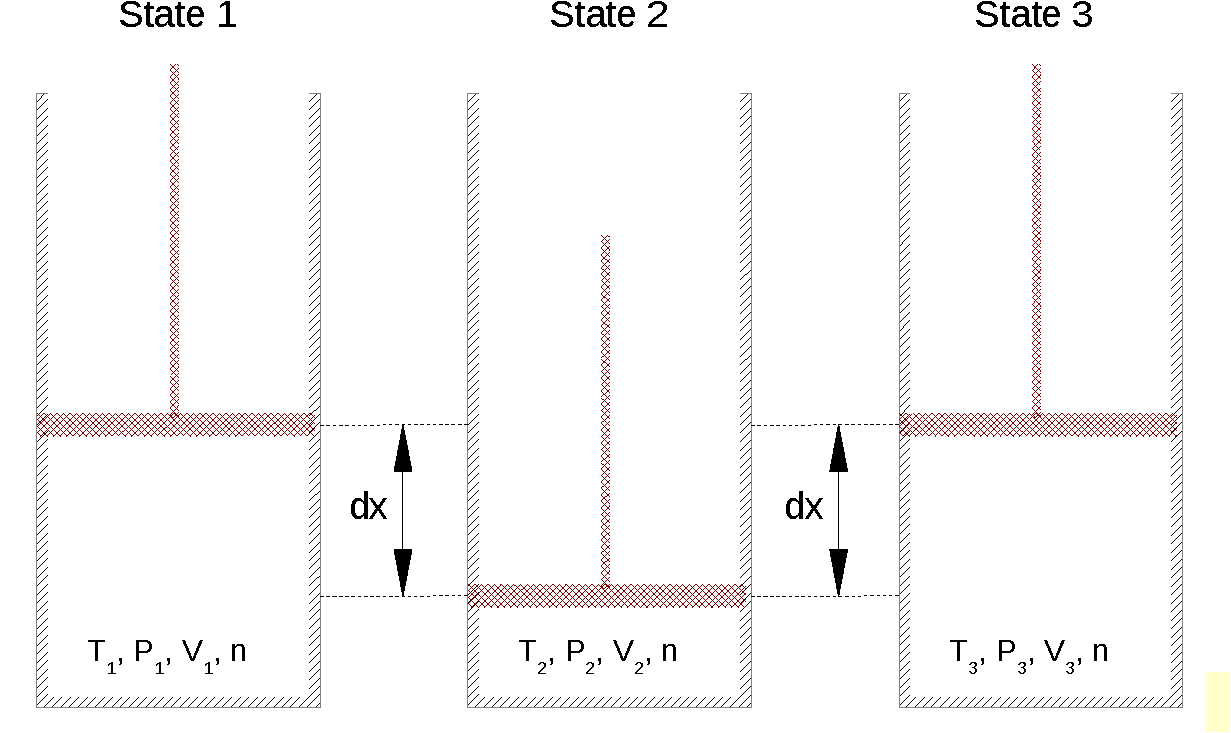
\includegraphics[width=0.7\columnwidth,clip]{./../Pics/Fig_SystemDefinition3}}
             \vspace{.1cm}
              \hbox{\hspace{8cm}(c)}}
        \label{Chapter:Introduction:Fig:Domain}
        \caption{System and control volumes: (a,b) schematics of systems and associated borders, (c) cylinder-piston system with extensive/intensive properties.}
      \end{figure}


      \begin{tabular}{|c|c|c|}
         \hline
                      & {\bf Mass} & {\bf Energy} \\
                      & {\bf Exchange} & {\bf Exchange} \\
         \hline
         {\bf Open}   & {\it yes}  & {\it yes}    \\
         {\bf Closed} & {\it no}   & {\it yes}    \\
         {\bf Isolated}&{\it no}   & {\it no}     \\
         \hline 
      \end{tabular}    

%%%
%%% SECTION
%%%
\section{Laws of Thermodynamics}\label{Chapter:Introduction:Section:LawsThermodynamics}\index{Laws of Thermodynamics}

%%%
%%% SECTION
%%%
\section{Zeroth Law}\label{zeroth_law}\index{Laws of Thermodynamics!Zeroth law}



%%%
%%% SECTION
%%%
\section{First Law}\label{first_law}\index{Laws of Thermodynamics!First law}


%%%
%%% SECTION
%%%
\section{Second Law}\label{second_law}\index{Laws of Thermodynamics!Second law}





blablabla \cite{batchelor_1967} \cite{SmithVanNess_Book}
\index{Reynolds Transport theorem}

\begin{exmp}
This is the example.
\end{exmp}
%%%
%%%  BIBLIOGRAPHY
%%%
%\bibliography{refbib}
